In this chapter we present the guidelines of designing a PREcision Timed (PRET) Machine. 
It is important to understand why and how current architectures fall short of timing predictability and repeatability.
Thus, we first discuss common architectural designs and their effects on execution time, and point out some key issues and trade-offs when designing architectures for predictable and repeatable timing.

\section{Pipelines}
The introduction of pipelining vastly improved the average-case performance of programs.
It allows faster clock speeds, and improves instruction throughput compared to single cycle architectures.
Pipelining begin executing subsequent instructions while prior instructions are still in execution. 
Ideally each processor cycle one instruction completes and leaves the pipeline as another enters and begins execution. 
In reality, different pipeline hazards occur which reduce the throughput and create stalls in the pipeline.
Different techniques were introduced to handle the effects of pipeline hazards, and greatly effect to the timing predictability and repeatability of an architecture.     
To illustrate this point, we discuss some basic hardware additions proposed to reduce performance penalty from hazards, and show how they effect the execution time and predictability. 

\subsection{Pipeline Hazards}
\begin{wrapfigure}{r}{0.5\textwidth}
  \vspace{-20pt}
  \begin{center}
    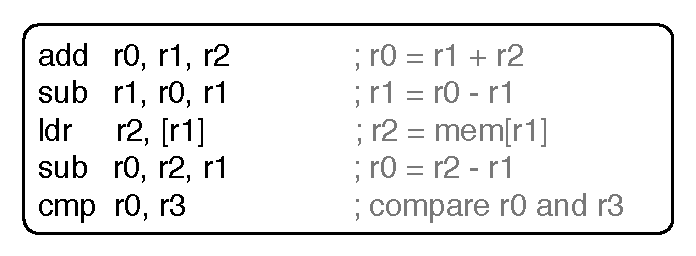
\includegraphics[scale=.65]{figs/sample_data_dependent_code}
  \end{center}
  \vspace{-20pt}
  \caption{Sample code with data dependencies}
  \label{fig:sample_data_dependent_code}
\end{wrapfigure}
Data hazards occur when instructions need the results of previous instructions that have not yet committed.
The code segment shown in figure~\ref{fig:sample_data_dependent_code} contains instructions that each depend on the result of its previous instruction.
Figure~\ref{fig:data_depend_execution_non_interleaved} shows two ways data hazards can be handled in a single-threaded pipeline. 
In the figure, time progresses horizontally towards the right, each time step, or column, represents a processor cycle.
Each row represents an instruction that is fetched and executed within the pipeline.
Each block represents the instruction entering the different stages of the pipeline -- fetch (F), decode (D), execute (E), memory (M) and writeback (W).   
The pipelines here are assumed to have a similar design to the five stage pipeline mentioned in Hennessy and Pattern~\todo{cite hennessy and patterson}.

A simple but effective way of handling data hazards is by simply stalling the pipeline until the previous instruction completes.
% Data hazards in this case are handled by inserting pipeline delays to ensure the completion of all dependent instructions.
%Similar to inserting pipeline delays of control-flow hazards, this method allows for predictable static execution time analysis, but at a slight cost of performance. 
%Figure~\ref{fig:data_depend_execution_non_interleaved} shows the execution of the code segment on pipelines with and without forwarding.
This is shown in the top of figure~\ref{fig:data_depend_execution_non_interleaved}. 
Pipeline delays (or bubbles) are inserted for instructions to wait until the previous instruction is complete.
The dependencies between instructions are shown in the figure to make clear why the pipeline bubbles are necessary.
The performance penalty incurred in this case is the pipeline delays inserted to wait for the previous instruction to complete.
Data forwarding was introduced to remove the need for inserting bubbles into the pipeline.
Data forwarding relies on the fact that the results of the previous instruction is typically available before the it commits.  
%Data forwarding is the most common way of handling data hazards that occur from pipelining.  
A data forwarding circuitry consists of backwards paths for data from later pipeline stages to the inputs of earlier pipeline stages, and multiplexers to select amongst all data signals. 
Because it provides a way to directly access computation results from the previous instruction before the previous instruction finishes, it removes the need to wait for the previous instruction to commit.  
The pipeline controller dynamically detects whether a data-dependency exists, and changes the selection bits to the multiplexers accordingly so the correct operands are selected.
The bottom of figure~\ref{fig:data_depend_execution_non_interleaved} shows the execution with forwarding in the pipeline.
\begin{figure}
\vspace{-20pt}
\begin{center}
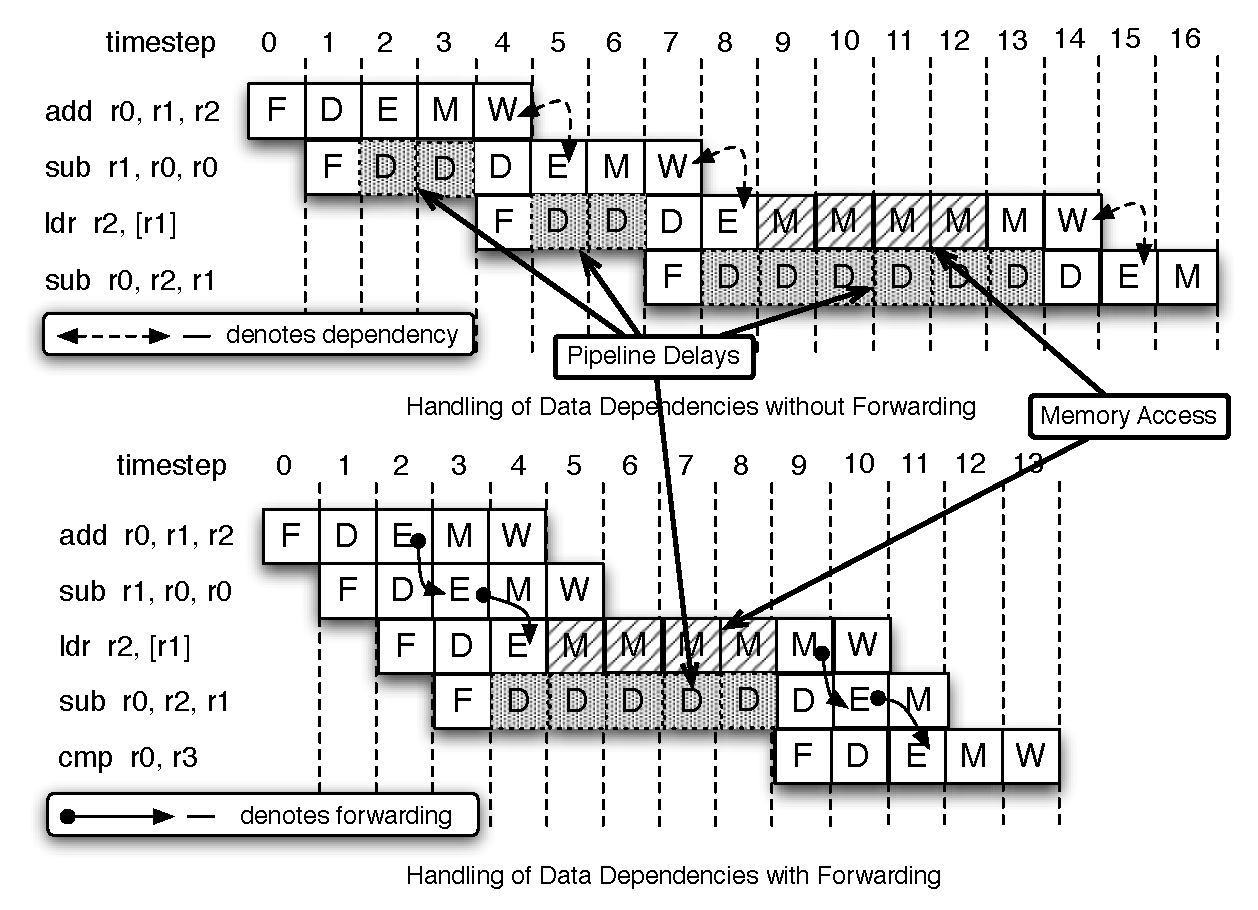
\includegraphics[scale=.6]{figs/data_depend_execution_non_interleaved}
\end{center}
\vspace{-10pt}
\caption{Handling of data dependencies in single threaded pipelines}
\label{fig:data_depend_execution_non_interleaved}
\end{figure}
No pipeline bubbles are needed for the first \emph{sub} instruction and \emph{ld} instruction because the data they depend on are forwarded with the forwarding paths.
However, the second \emph{sub} instruction after the \emph{ld} instruction still stalls. 
As mentioned earlier, forwarding relies on the results from the previous instruction being available before the previous instruction commits. 
In the case of longer latency operations, such as memory accesses, the data cannot be forwarded until it becomes available, so stalls are still required.
The memory access latency in the figure is arbitrarily chosen to be 5 cycles so the figure is not too long and instructions after the \emph{ld} instruction can be shown.  
We purposely leave out the details regarding memory accesses at this point, and will discuss it extensively in section~\ref{section:memory_system}.
We merely use the \emph{ld} instruction to illustrate the limitations of data forwarding.
They can address the data-dependencies caused by pipelining -- the read-after-write of register computations. 
However, they cannot address the data-dependencies caused by other long latency operations such as memory operations, so pipeline stalls are still needed.
More involved techniques such as the introduction of out-of-order execution or superscalar pipelines are used to mitigate the effects of long latency operations. 
We will discuss more of these in chapter~\ref{chapter:related} when we mention the related works.  

To understand the timing effects of handling data hazards, we discuss how to determine execution time for instructions using both methods of handling data hazards.  
With the simple method of inserting stalls, we need to know when the stalls will be inserted and how long the instruction will need to stall for.
This information can be determined by simply checking the previous instruction since stalls are inserted only if this instruction depends on the results of the previous instruction.
Within pipelines, the execution of most instructions are deterministic, so for the most part we can determine how long the stall will be by
checking the previous instruction.
Memory access instructions are an exception to instructions that have deterministic execution time, but as mentioned before, we will discuss these extensively in section~\ref{section:memory_system}.
For pipelines with data forwarding, we need to know in what situations the data forwarding circuitry cannot correctly forward the data to the next instruction.    
Although the pipeline dynamically forwards the data during run-time, the logic in the pipeline controller that enables and selects the correct forwarding bits only needs to keep track of a small set of previous instructions to detect data-dependencies.
The set of instructions it needs to check usually depends on the depth of the pipeline.  
Thus, static execution time analysis can detect forwarding by simply checking a short window of previous instructions to account for stalls accordingly. \todo{find papers to back this up}
We simplified greatly the execution time analysis discussed above to ignore effects from other pipeline mechanisms.
We wanted to simply focused on the effects of handling data-hazards through stalling or data-forwarding.  
We can see that both methods of handling data-hazards cause instruction execution time to depend previous instruction execution history. 
But the execution history that instruction execution time is dependent upon is small and temporary enough to be accounted for.
  
%The internal state of the branch predictor on the other hand is dependent on branch histories which may have happened arbitrarily long ago in the execution sequence,
%\todo{more complicated ways of handling data hazards include out-of-order execution\ldots}  

\begin{wrapfigure}{r}{0.5\textwidth}
  \vspace{-20pt}
  \begin{center}
    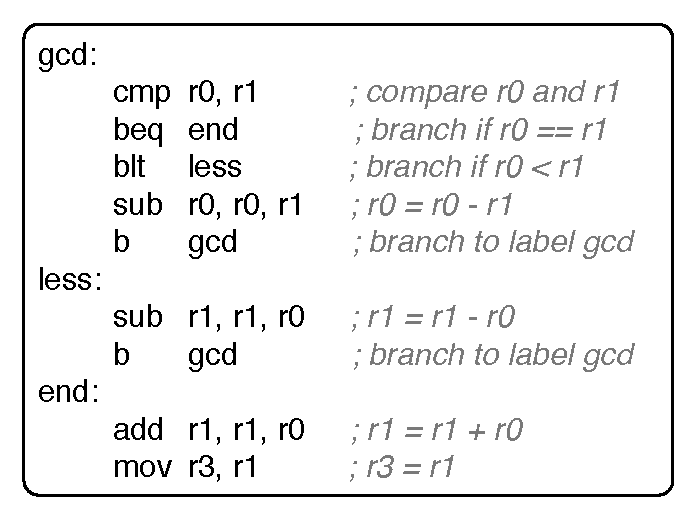
\includegraphics[scale=.65]{figs/sample_gcd_code}
  \end{center}
  \vspace{-20pt}
  \caption{Sample code for GCD with conditional branches}
  \label{fig:sample_gcd_code}
\end{wrapfigure}
Branches cause control-flow hazards in the pipeline; the instruction after the branch, which should be fetched the next cycle, is unknown until after the branch instruction is completed.
Conditional branches further complicates matters, as whether or not the branch is taken depends on an additional condition that could possible be unknown when the conditional branch is in execution. 
The code segment in figure~\ref{fig:sample_gcd_code} shows assembly instructions from the ARM instruction set architecture (ISA) that implement the Greatest Common Divisor (GCD) algorithm using conditional branch instructions \emph{beq} (branch equal) and \emph{blt} (branch less than).  
Conditional branch instructions in ARM branch based on conditional bits that are stored in a processor state register and set with special compare instructions\todo{cite arm manual}.
The \emph{cmp} instruction is one such compare instruction that subtracts two registers and sets the conditional bits according to the results.
The GCD implementation shown in the code uses this mechanism to determine whether to continue or end the algorithm.
Figure~\ref{fig:branch_execution_non_interleaved_pipeline} show two ways branches can be handled in a single-threaded pipeline. 

\begin{figure}
\begin{center}
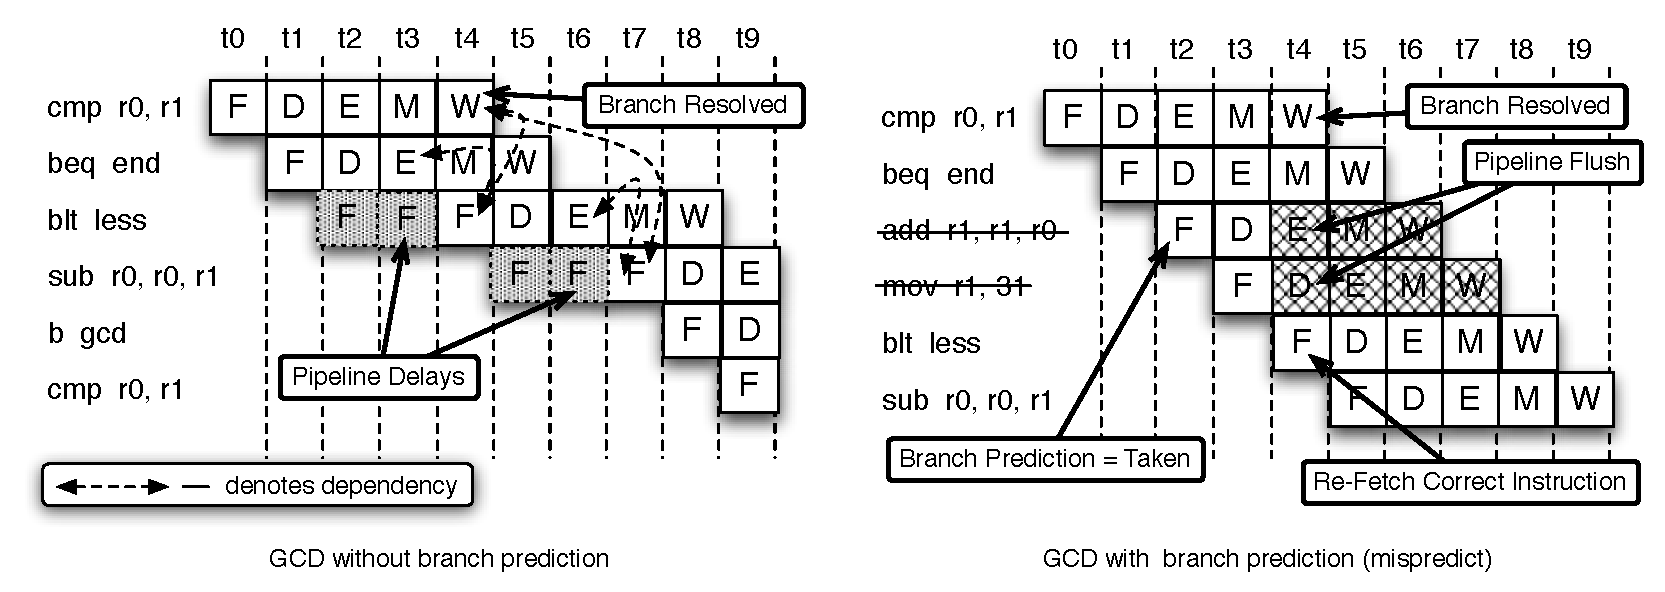
\includegraphics[scale=.58]{figs/branch_execution_non_interleaved_pipeline}
\end{center}
\vspace{-10pt}
\caption{Handling of conditional branches in single threaded pipelines}
\label{fig:branch_execution_non_interleaved_pipeline}
\end{figure}
Similar to handling data-hazards, a simple but effective way of handling control-flow hazards is by simply stalling the pipeline until the branch instruction completes.
This is shown on the left of figure~\ref{fig:branch_execution_non_interleaved_pipeline}. 
Two pipeline delays (or bubbles) are inserted after each branch instruction to wait until address calculation is completed.
The dependencies between instructions are also drawn out to make clear why the pipeline bubbles are necessary.
In order for the \emph{blt} instruction to be fetched, its address must be calculated during the execution stage of the \emph{beq} instruction.
At the same time, because \emph{beq} is a conditional branch, whether or not the branch is taken depends on the \emph{cmp} instruction.
The pipeline here is assumed to have forwarding circuitry, so the addresses calculated by the branch instructions and the results of the \emph{cmp} instruction can be used before the instructions are committed.
The performance penalty incurred is the pipeline delays inserted to wait for the branch address calculation to complete.
Conditional branches will also incur extra delays for deeper pipelines if the branch condition cannot be resolved in time. 
Some architectures enforce the compiler to insert one or more non-dependent instructions after a branch that is always executed before the change in control-flow of the program. 
These are called branch delay slots and can mitigate the branch penalty, but become less effective as pipelines grow deeper because the longer delay slots are required.  

In attempt to remove the need of inserting pipeline bubbles, branch predictors were invented to predict the results of a branch before it is resolved\todo{citation}.
%Branch predictors have been heavily researched.
Many clever branch predictors have been proposed, and they can accurately predict branches up to 93.5\%\todo{citation}.
%With branch predictor, the pipeline fetches the next instruction based upon the results of the branch prediction, and continues to execute speculatively.
Branch predictors predict the condition and target addresses of branches, so pipelines can speculatively continue execution based upon the prediction.  
If the prediction was correct, no penalty occurs for the branch, and execution simply continues. 
However, when a mispredict occurs, then the speculatively executed instructions need to be flushed and the correct instructions need to be refetched into the pipeline for execution.
The right of figure~\ref{fig:branch_execution_non_interleaved_pipeline} shows the execution of GCD in the case of a branch misprediction.
After the \emph{beq} instruction, the branch is predicted to be taken, and the \emph{add} and \emph{mov} instructions from the label \emph{end} is directly fetched into execution. 
When the \emph{cmp} instruction is completed, a misprediction is detected, so the \emph{add} and \emph{mov} instruction are flushed out of the pipeline while the correct instruction \emph{blt} is immediately re-fetched and execution continues.
The misprediction penalty is typically the number of stages between fetch and execute, as those cycles are wasted executing instructions from an incorrect execution path.
This penalty only occurs on a mispredict, thus branch prediction typically yields better average performance and is preferred for modern architectures.
%However, for more complex architectures with caches or other hardware states, the effects of incorrectly fetched instructions on the state of the processor less well-known and studied. 
Nonetheless, it is important to understand the effects of branch prediction on execution time. 

Typical branch predictors predict branches based upon the history of previous branches encountered.  
As each branch instruction is resolved, the internal state of the predictor, which stores the branch histories, is updated and used to predict the next branch.
This implicitly creates a dependency between branch instructions and their execution history, as the prediction is affected by its history.
In other words, the execution time of a branch instruction will depend on the branch results of previous branch instructions.
During static execution timing analysis, the state of the branch predictor is unknown because is it often infeasible to keep track of execution history so far back.   
There has been work on explicitly modeling branch predictors for execution time analysis\todo{citation}, but the results are \todo{the results of branch predictor modeling for execution time analysis}.
The analysis needs to conservatively account for the potential branch mispredict penalty for each branch, which leads to overestimated execution times.
To make matters worse, as architectures grow in complexity, more internal states exist in architectures that could be affected by the speculative execution. 
For example, cache lines could be evicted when speculatively executing instructions from a mispredicted path, changing the state of the cache.  
%When instructions from the correct execution path are re-fetched at branch resolution, a cache miss could be resulted from the change in cache because of the branch misprediction.    
This makes a tight static execution time analysis extremely difficult, if not impossible; explicitly modeling all hardware states and their effects together often lead to an infeasible explosion in state space. 
On the other hand, although the simple method of inserting pipeline bubbles for branches could lead to more branch penalties, the static timing analysis is precise and straight forward, as no prediction and speculative execution occur. 
The timing analysis simply adds the branch penalty to the instruction after a branch. 
Additional penalties from a conditional branch can be accounted for by simply checking for instructions that modify the conditional flag above the conditional branch.
We explicitly showed this simple method of handling branches to point out an important trade-off between speculative execution for better average performance and consistent stalling for better predictability.
Average-case performance can be improved by speculation at the cost of predictability and potentially prolonging the worst-case performance.  
The challenge remains to maintain predictability while improving worst-case performance, and how pipeline hazards are handled play an integral part of tackling this challenge.           

\subsection{Pipeline Multithreading}
 Multithreaded architectures were introduced to improve instruction throughput over instruction latency.
The architecture optimizes thread-level parallelism over instruction-level parallelism to improve performance.
Multiple hardware threads are introduced into the pipeline to fully utilize thread-level parallelism. 
When one hardware thread is stalled, another hardware thread can be fetched into the pipeline for execution to avoid stalling the whole pipeline. 
To lower the context switching overhead, the pipeline contains physically separate copies of hardware thread states, such as registers files and program counters etc, for each hardware thread.
\begin{figure}
\begin{center}
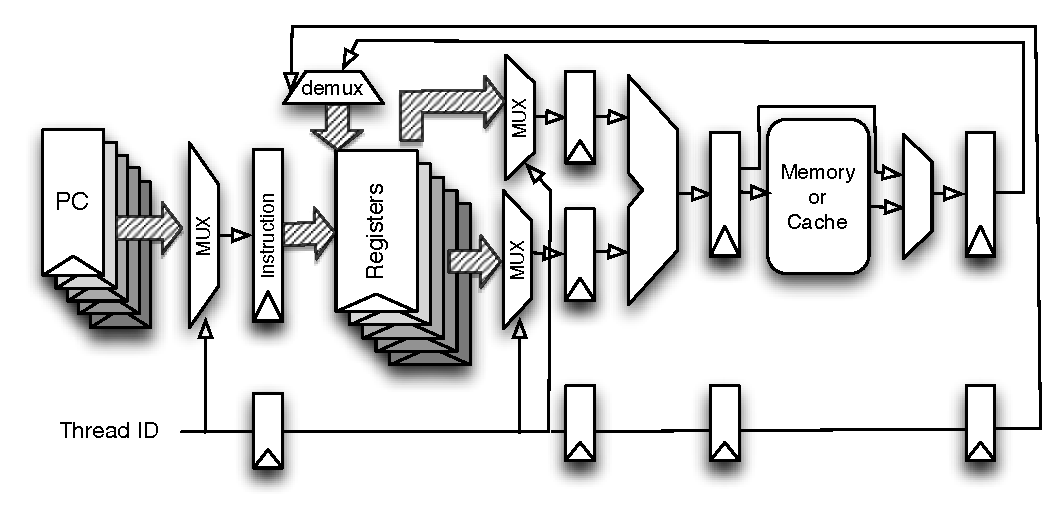
\includegraphics[scale=.8]{figs/multithreaded_pipeline_block}
\end{center}
\vspace{-30pt}
\caption{Simple Multithreaded Pipeline}
\label{fig:multi-thread pipeline simplified}
\end{figure}
Figure~\ref{fig:multi-thread pipeline simplified} shows a architectural level view of a simple multithreaded pipeline.
It contains 5 hardware threads, so it has 5 copies of the Program Counter (PC) and Register files.
Once a hardware thread is executing in the pipeline, its corresponding thread state can be selected by signaling the correct selection bits to the multiplexers.
The rest of the pipeline remains similar to a traditional 5 stage pipeline as introduced in Hennessy and Pattern\todo{citation}.   
The extra copies of the thread state and the multiplexers used to select them thus contribute to most of the hardware additions needed to implement hardware multithreading.

%The selection of threads for execution is one of the most important factors to fully utilize thread-level parallelism.
%If a thread is stalled waiting for memory access but gets selected to execute in the pipeline, then that instruction slot is wasted and the processor isn't fully utilized.
Ungerer et al.~\cite{Ungerer:2003:survey_multithreading} surveyed different multithreaded architectures and categorized them based upon the \todo{thread selection?} policy and the execution width of the pipeline.
The thread selection policy is the context switching scheme used to determine which threads are executing, and how often a context switch occurs.  
Coarse-grain policies manage hardware threads similar to the way operation systems manage software threads.
A hardware thread gain access to the pipeline and continues to execute until a context switch is triggered.
Context switches occur less frequently via this policy, so less hardware threads are required to fully utilize the processor.
Different coarse-grain policies trigger context switches with different events. 
Some trigger on dynamic events, such as cache miss or interrupts, and some trigger on static events, such as specialized instructions.
Fine-grain policies switch context much more frequently -- usually every processor cycle.
Both coarse-grain and fine-grain policies can also have different hardware thread scheduling algorithms that are implemented in a hardware thread scheduling controller to determine which hardware thread is switched into execution.  
The width of the pipeline refers to the number of instructions that can be fetched into execution in one cycle. 
For example, superscalar architectures have redundant functional units, such as multipliers and ALUs, and can dispatch multiple instructions into execution in a single cycle. 
Multithreaded architectures with pipeline widths of more than one, such as Sumultanous Multithreaded (SMT) architectures, can fetch and execute instructions from several hardware threads in the same cycle.

Multithreaded architectures typically bring additional challenges to execution time analysis of software running on them.
Any timing analysis for code running on a particular hardware thread needs to take into account not only the code itself, but also the thread selection policy of the architecture and sometimes even the execution context of code running on other hardware threads.
For example, if dynamic coarse-grain multithreading is used, then a context switch could occur at any point when a hardware thread is executing in the pipeline.
This not only has an effect on the control flow of execution, but also the state of any hardware that is shared, such as caches or branch predictors.    
Thus, it becomes nearly impossible to estimate execution time without knowing the exact execution state of other hardware threads and the state of the thread scheduling controller.
However, it is possible to for multithreaded architectures to fully utilize thread-level parallelism while still maintaining timing predictability.
Thread-interleaved pipelines use a fine-grain thread switching policy with round robin thread scheduling to achieve high instruction throughput while still allowing precise timing analysis for code running on its hardware threads. 
Below, its architecture and trade-offs are described and discussed in detail along with examples and explanation of how timing predictability is maintained.
Through the remainder of this chapter, we will use the term ``thread'' to refer to explicit hardware threads that have physically separate register files, program counters, and other thread states.
This is not to be confused the common notion of ``threads'', which is assumed to be software threads that is managed by operating systems with thread states stored in memory.

\subsection{Thread-Interleaved Pipelines}
\label{section:pret_thread_pipeline}
\todo{Go through and make sure you don't say minimum threads as pipeline stages is a requirement, since later we have 4 threads in a give stage pipeine.}
\begin{figure}
  \vspace{-20pt}
  \begin{center}
    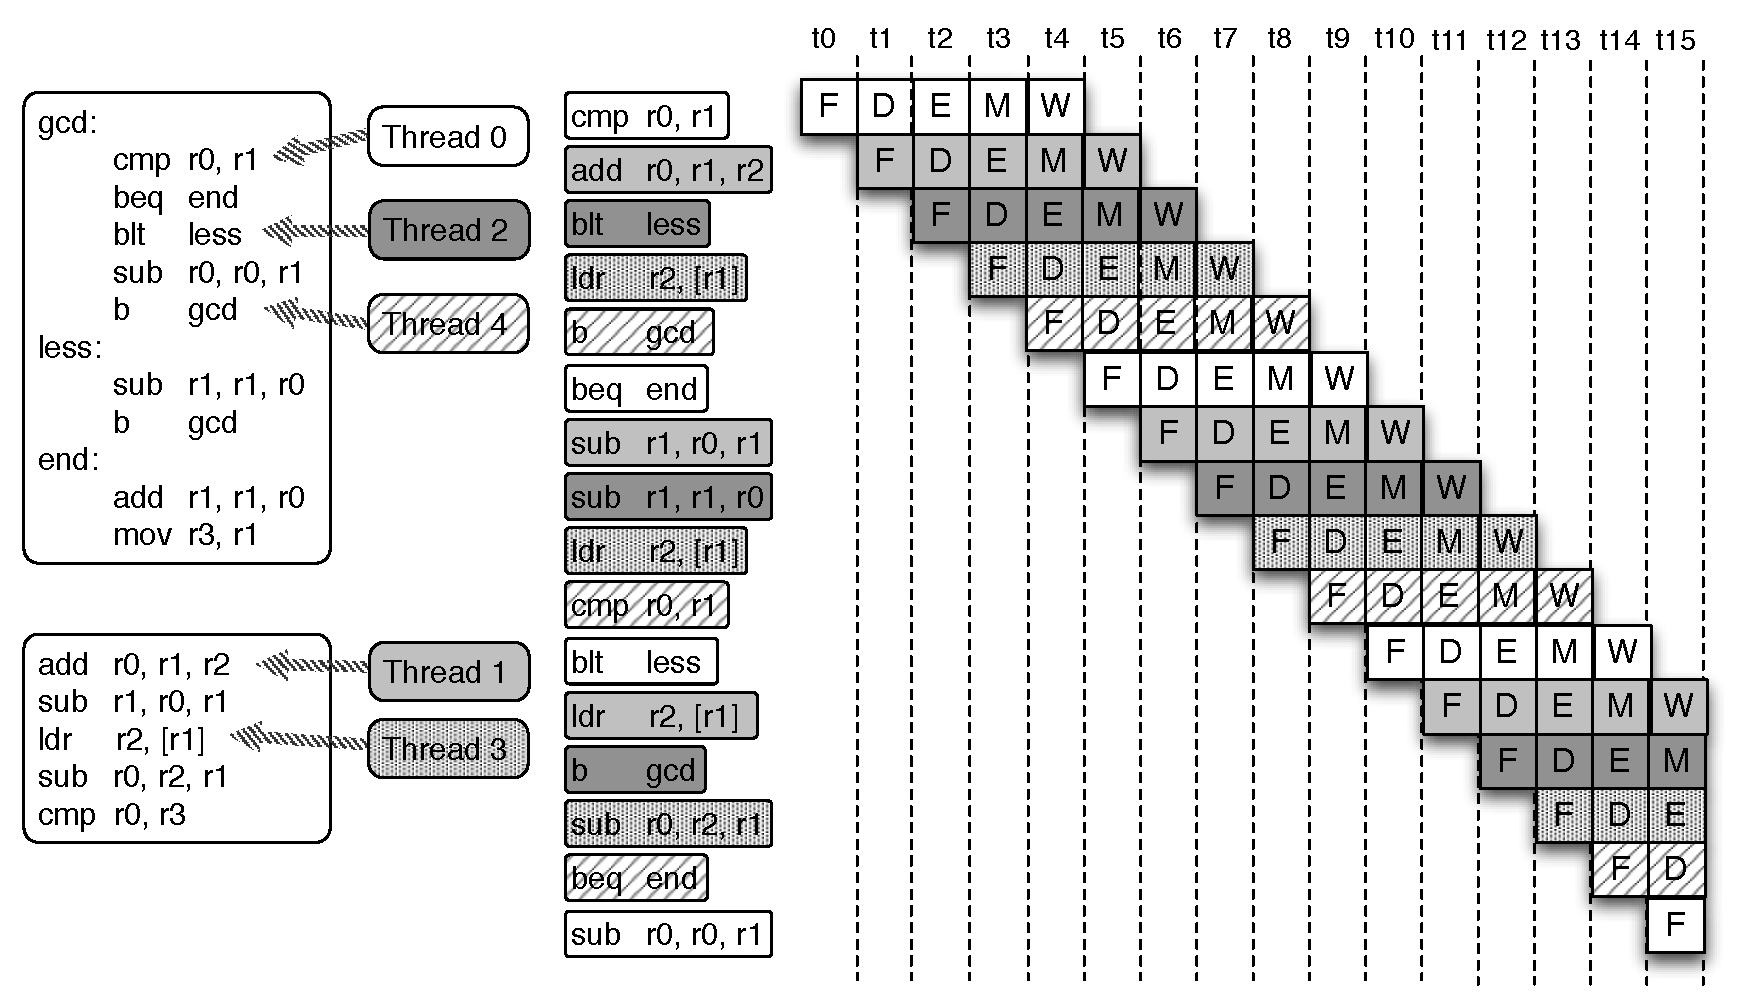
\includegraphics[scale=.55]{figs/thread-interleaved-execution}
  \end{center}
  \vspace{-20pt}
  \caption{Sample execution sequence of a thread-interleaved pipeline with 5 threads and 5 pipeline stages}
  \label{fig:execution_thread_interleaved_pipeline}
\end{figure}
The thread-interleaved pipeline was introduced to improve the response time of handling multiple I/O devices \todo{citation}.
I/O operations often stall from the communication with the I/O devices.
Thus, interacting with multiple I/O devices leads to wasted processor cycles that are idle waiting for the I/O device to respond.
By employing multiple hardware thread contexts, a hardware thread stalled from the I/O operations does not stall the whole pipeline, as other hardware threads can be fetched and executed.
% In a thread-interleaved pipeline, a thread context switch occurs every processor cycle, and the threads are cycled through in a round robin fashion. 
% This ensures each thread gets equal access to the process resource, so threads that aren't stalled are guaranteed to make progress.
Thread-interleaved pipelines use fine-grain multithreading; every cycle a context switch occurs and a different hardware thread is fetched into execution. 
The threads are scheduled in a deterministic round robin fashion. 
This also reduces the context switch overhead down to nearly zero, as no time is needed to determine which thread to fetch next.
Barely any hardware is required to implement round robin thread scheduling; a simple $log(n)$ bit up counter (for $n$ threads) would suffice.         
Figure~\ref{fig:execution_thread_interleaved_pipeline} shows an example execution sequence from a 5 stage thread-interleaved pipeline with 5 threads.
The thread-interleaved pipelines shown and presented in this thesis are all of single width.
The same code segments from figure~\ref{fig:sample_gcd_code} and figure~\ref{fig:sample_data_dependent_code} are being executed in this pipeline. 
Threads 0, 2 and 4 execute GCD (figure~\ref{fig:sample_gcd_code}) and threads 1 and 3 execute the data dependent code segment (figure~\ref{fig:sample_data_dependent_code}).
Each hardware thread executes as an independent context and their progress is shown in figure~\ref{fig:execution_thread_interleaved_pipeline} with thick arrows pointing to the execution location of each thread at t0.
We can observe from the figure that each time step an instruction from a different hardware thread is fetched into execution and the hardware threads are fetched in a round robin order.
At time step 4 we begin to visually see that each time step, each pipeline stage is occupied by a different hardware thread.
The fine-grained thread interleaving and the round robin scheduling combine to form this important property of thread-interleaved pipelines, which provides the basis for a timing predictable architecture design.

For thread-interleaved pipelines, if there are enough thread contexts, for example -- the same number of threads as there are pipeline stages, then at each time step no dependency exists between the pipeline stages since they are each executing on a different thread. 
As a result, data and control pipeline hazards, the results of dependencies between stages within the pipelines, no longer exist in the thread-interleaved pipeline.    
We've already shown from figure~\ref{fig:branch_execution_non_interleaved_pipeline} that when executing the GCD code segment on a single-threaded pipeline, control hazards stem from branch instructions because of the address calculation for the instruction after the branch.
However, in a thread-interleaved pipeline, the instruction after the branch from the same thread is not fetched into the pipeline until the branch instruction is committed.
Before that time, instructions from other threads are fetched so the pipeline is not stalled, but simply executing other thread contexts.
This can be seen in figure~\ref{fig:execution_thread_interleaved_pipeline} for thread 0, which is represented with instructions with white backgrounds.
The \emph{cmp} instructions, which determines whether next conditional branch \emph{beq} is taken or not, completes before the \emph{beq} is fetched at time step 5.
The \emph{blt} instruction from thread 0, fetched at time step 10, also causes no hazard because the \emph{beq} is completed before \emph{blt} is fetched.
The code in figure~\ref{fig:sample_data_dependent_code} is executed on thread 1 of the thread interleave pipeline in figure~\ref{fig:execution_thread_interleaved_pipeline}.
The pipeline stalls inserted from top of figure~\ref{fig:data_depend_execution_non_interleaved} are no longer needed even without a forwarding circuitry because the data-dependent instructions are fetched after the completion of its previous instruction.
In fact, no instruction in the pipeline is dependent on another because each pipeline stage is executing on a separate hardware thread context.
Therefore, the pipeline does not need to include any extra logic or hardware for handling data and control hazards in the pipeline. 
This gives thread-interleaved pipelines the advantage of a simpler pipeline design that requires less hardware logic, which in turns allows the pipeline clock speed to increase.
Thread-interleaved pipelines can be clocked at higher speeds since each pipeline stage contains significantly less logic needed to handle hazards.
The registers and processor states use much more compact memory cells compared to the logic and muxes used to select and handle hazards, so the size footprint of thread-interleaved pipelines are also typically smaller.

For operations that have long latencies, such as memory operations or floating point operations, thread-interleaved pipelines hides the latency with its execution of other threads. 
Thread 3 in figure~\ref{fig:execution_thread_interleaved_pipeline} shows the execution of a \emph{ld} instruction that takes the same 5 cycles as shown in figure~\ref{fig:data_depend_execution_non_interleaved}.
We again assume that this \emph{ld} instruction accesses data from the main memory. 
While the \emph{ld} instruction is waiting for memory access to complete, the thread-interleaved pipeline executes instructions from other threads.
The next instruction from thread 3 that is fetched into the pipeline is again the same \emph{ld} instruction.  
As memory completes its execution during the execution of instructions from other threads, we replay the same instruction to pick up the results from memory and write it into registers to complete the execution of the \emph{ld} instruction. 
It is possible to directly write the results back into the register file when the memory operation completes, without cycling the same instruction to pick up the results.
This would require hardware additions to support and manage multiple write-back paths in the pipeline, and a multi write ported register file, so contention can be avoided with the existing executing threads.
In our design we simply replay the instruction for write-backs to simplify design and piggy back on the existing write-back datapath.
%We showed a memory access instruction in our example, but the same reasoning is applied to floating point instructions or any long latency instruction.  
Multithreaded pipelines typically mark threads inactive when they are waiting for long latency operations.
Inactive threads are not fetched into the pipeline, since they cannot make progress even if they are scheduled. 
This allows the processor to maximize throughput by allowing other threads to utilize the idle processor cycles.   
However, doing so has non-trivial effects on thread-interleaved pipelines and the timing of other threads. 

First, if the number of ``active'' threads falls below the number of pipeline stages, then pipeline hazards are reintroduced; it is now possible for the pipeline to be executing two instructions from the same thread that depend on each other simultaneously. 
This can be circumvented by inserting pipeline bubbles when there aren't enough active threads. 
For example, as shown in figure~\ref{fig:three_thread_pipeline}, for our 5 stage thread-interleaved pipeline that has 5 threads, if two threads are waiting for main memory access and are marked inactive, then we insert 2 NOPs every round of the round-robin schedule to ensure that no two instructions from the same thread exists in the pipeline.
Note that if the 5 stage thread-interleaved pipeline contained 7 threads, then even if 2 threads are waiting for memory, no NOP insertion would be needed since instructions in each pipeline stage in one cycle would still be from a different thread.   
NOP insertions only need to occur when the number of active threads drops below the number of pipeline stages.   
\begin{figure}
  \vspace{-20pt}
  \begin{center}
    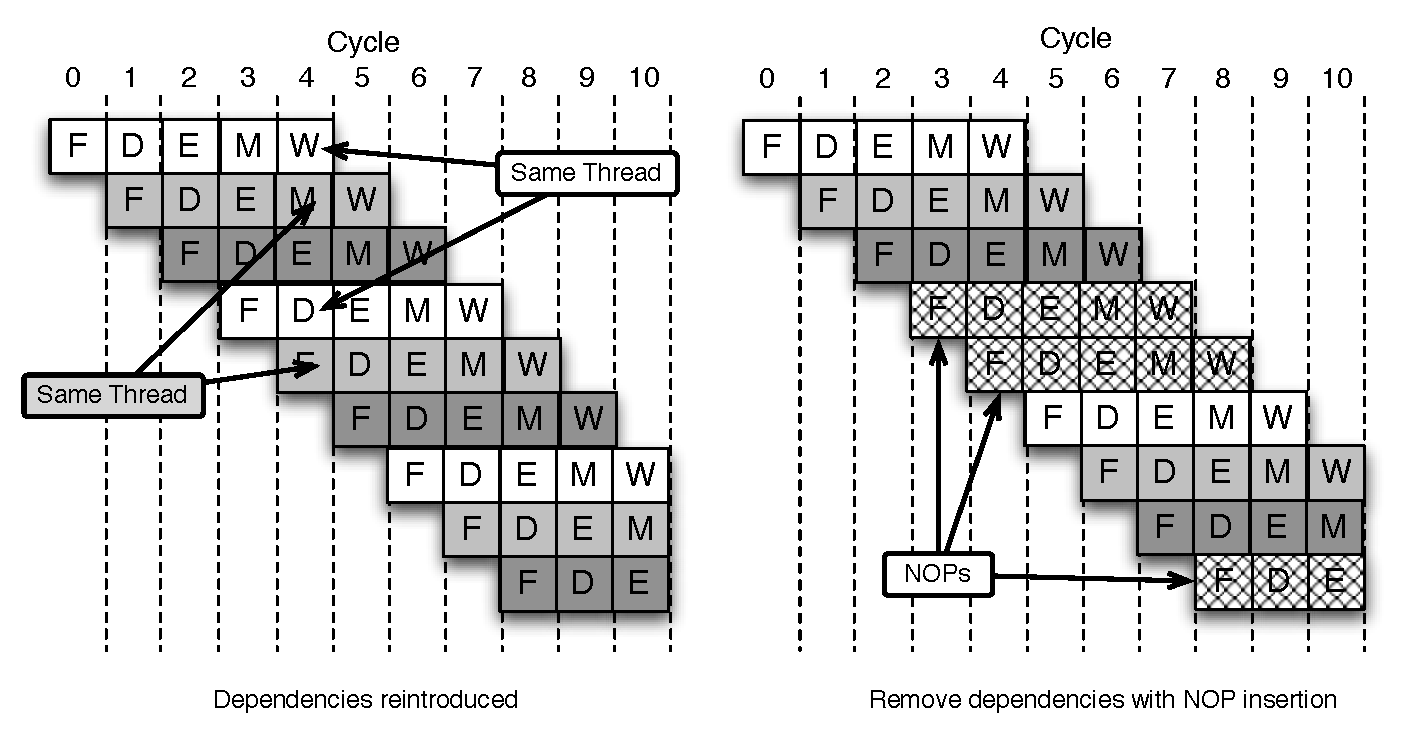
\includegraphics[scale=.6]{figs/three_thread_pipeline}
  \end{center}
  \vspace{-20pt}
  \caption{Execution of 5 threads thread-interleaved pipeline when 2 threads are inactive}
  \label{fig:three_thread_pipeline}
\end{figure}

The more problematic issue with setting threads inactive whenever long latency operations occur is the effect on the execution frequencies of other threads in the pipeline.
When threads are scheduled and unscheduled dynamically, the other threads in the pipeline would dynamically execute more or less frequently depending on how many threads are active.
This complicates timing analysis since the thread frequency of one thread now depends on the program state of all other threads. 
In order for multithreaded architectures to achieve predictable performance, \emph{temporal isolation} must exist in the hardware between the threads.
Temporal isolation is the isolation of timing behaviors of a thread from other thread contexts in the architecture.
For example, if a multithreaded architecture shares a branch predictor amongst all threads, and the branch table entries can be overwritten by branches from other threads in the pipeline, then each thread's branches can cause a branch mispredict for any other thread. 
Also as mentioned above, dynamically scheduling and unscheduling threads also breaks temporal isolation amongst threads.
With temporal isolation, the timing analysis is greatly simplified, as software running on individual threads can be analyzed separately without worry about the effects of integration. 
If temporal isolation is broken, any timing analysis needs to model and explore all possible combinations of program state of all threads, which is typically infeasible.
The round-robin thread scheduling of thread-interleaved pipelines is a way of achieving temporal isolation for a multithreaded architecture.
Unlike coarse-grain dynamically switched multithreaded architectures, thread-interleaved pipelines can maintain the same round-robin thread schedule despite the execution context of each thread within the pipeline. 
This is a step towards achieving temporal isolation amongst the threads, as the execution frequency of threads does not change dynamically.  
Thus, our thread-interleaved pipeline does not mark threads inactive on long latency operations, but simply replays the instruction whenever the thread is fetched.  
Although this slightly reduces the utilization of the thread-interleaved pipeline, but threads are decoupled and timing analysis can be done individually for each thread without interference from other threads.
At the same time, we still preserve some of the benefits of latency hiding, as other threads are still executing during the long latency operation.

Thread-interleaved pipelines however still contain structural hazards, hazards that occur when hardware units are needed by two or more instructions at the same time.
Although each pipeline stage is occupied by different hardware threads, two or more threads can simultaneously be issuing \emph{ld} instructions to the main memory.
If the shared main memory can only handle one request at a time, then the second request must be queued waiting for the first requester to complete.
This creates timing interference between the threads, because the memory access time of a memory request from a particular thread now depends on if the memory is currently being access by other threads, and how many threads are already queued up.
We will discuss how our redesigned memory controller supports pipelining memory access in section~\ref{section:memory_system}, but the same hazard applies to any shared hardware unit such as floating point units etc.
If the hardware unit can be pipelined and accept inputs every cycle, then no contention arises between the hardware threads, and no structural hazards occur.
%FIXME: more explanation
If pipelining cannot be achieved, then any timing analysis of that instruction must include a conservative estimation that accounts for thread access interference.
A time division multiplex access (TDMA) schedule can be enforced to decouple the access time of threads to the shared hardware unit.
%FIXME: Explain TDMA scheduling  
  
It is important to understand that it is not the thread scheduling that is non-predictable, but how thread switches are triggered.    
It is still possible for a predictable architecture to support the scheduling of hardware threads, but it must be done statically in software, instead of dynamically in hardware. 
If the hardware can provide a means of explicitly setting thread schedules in software, then it is possible to make the thread schedules transparent to any timing analysis.	 
The software still needs to be carefully constructed, since it is still possible for the software to switch hardware thread schedules dynamically, complicating the timing analysis. 
One could envision a program that contains different program states, each state executing a different number of threads. 
As long as the state transitions are statically analyzable, the timing analysis complexity is not increased. 

%FIXME: Show a simple timing analysis of thread-interleaved pipelines and how easy it is, compare it to a timing analysis of single threads?
%FIXME: Talk about the trade-offs of threaded interleaved pipelines to summarize 
In summary, blah blah blah\ldots
\section{Memory System}
\label{section:memory_system}
\subsection{Scratchpad}
\subsection{DRAM memory controller}


